\chapter{Probability by Rosenthal}
In this chapter, I will include sporadic notes during my study of probability from the Rosenthal book. Also, I will try to compile a set of solutions for the problems in this book.



\section{Probability Triples}

\begin{definition}[Semialgebra]
	Let $ X $ be a set. A Semialgebra $ \mathcal{I} $ of the subsets of $ X $ is a collection of the subsets of such that 
	\begin{enumerate}[(a)]
		\item $ \emptyset, X \in \mathcal{I} $.
		\item $ \mathcal{I} $ is closed \emph{finite} \textbf{intersection}.
		\item For $ E \in \mathcal{I} $ it complement $ E^c $ can be written as a \emph{finite disjoint} \textbf{union} of sets in $ \mathcal{I} $.
	\end{enumerate}
\end{definition}
\begin{remark}
	One canonical example for a semialgebra is the set of all intervals in $ \R $, where the term interval contains all open, closed and half open intervals, as well as the empty set, singletons, and the whole space. 
\end{remark}

\begin{definition}[Algebra]
	Let $ \mathcal{M} $ be a collection of sets. Then $ \mathcal{M} $ is an algebra if 
	\begin{enumerate}[(a)]
		\item $ \Omega, \emptyset \in \mathcal{M} $
		\item $ \mathcal{M} $ is closed under complements.
		\item $ \mathcal{M} $ is closed under finite intersection.
		\item $ \mathcal{M} $ is closed under finite union.
	\end{enumerate}
\end{definition}

\begin{proposition}
	Let $ \mathcal{I} $ be a semialgebra, and $ \mathcal{F} = \sigma(\mathcal{I}) $. Let $ \mathbb{P},\mathbb{Q} $ be two probability measures defined on $ \mathcal{F} $. Then if $ \mathbb{P} $ agrees with $ \mathbb{Q} $ on $ \mathcal{I} $, then they agree on $ \mathcal{F} $.
\end{proposition}
\begin{remark}
	The condition that $ \mathcal{I} $ is a semialgebra is crucial. See \autoref{prob:BeingSemiAlgebraIsImportant} for an example.
\end{remark}


\newpage

\subsection{Solved Problems}
\begin{problem}
	Let $ \Omega = \set{1,.2,3,4} $. Determine whether or not each of the following is a $\sigma\text{-algebra}$.
	\begin{enumerate}[(a)]
		\item $ \mathcal{F}_1 = \set{\emptyset, \set{1,2},\set{3,4},\set{1,2,3,4}} $.
		\item $ \mathcal{F}_2 = \set{\emptyset,\set{3},\set{4},\set{1,2},\set{3,4},\set{1,2,3},\set{1,2,4},\set{1,2,3,4}} $.
		\item $ \mathcal{F}_3 = \set{\emptyset, \set{1,2},\set{1,3},\set{1,4},\set{2,3},\set{2,4},\set{3,4},\set{1,2,3,4}} $.
	\end{enumerate}
\end{problem}
\begin{solution}
	\begin{enumerate}[(a)]
		$ \, $
		\item $ \mathcal{F}_1  $ is a $\sigma\text{-algebra}$ and the set of its atoms are $ \set{\set{1,2},\set{3,4}} $. 
		\item $ \mathcal{F}_2 $ is a $\sigma\text{-algebra}$ and the set of its atoms are $ \set{\set{3},\set{4},\set{1,2}} $.
		\item $ \mathcal{F}_3 $ is \textbf{not} a $\sigma\text{-algebra}$ because $ \set{1,2},\set{2,3} \in \mathcal{F}_3 $ but $ \set{1,2}\cap\set{2,3} = \set{2} \notin \mathcal{F}_3 $.
 	\end{enumerate}
\end{solution}

\begin{problem}
	Let $ \Omega = \set{1,2,3,4} $, and let $ \mathcal{I} = \set{\set{1},\set{2}} $. Describe explicitly the $\sigma\text{-algebra}$ $ \sigma(\mathcal{I}) $ (i.e. the smallest $\sigma\text{-algebra}$ containing the collection $ \mathcal{I} $).
\end{problem}
\begin{solution}
	The smallest $\sigma\text{-algebra}$ containing the collection $ \mathcal{I} $ is
	\[ \sigma(\mathcal{I}) = \set{\set{1},\set{2},\set{3,4},\set{1,2},\set{2,3,4},\set{1,3,4},\set{1,2,3,4},\emptyset}. \]
	One way to check to see if this is really the smallest $\sigma\text{-algebra}$ is to first observe that the cardinality of $\sigma\text{-algebra}$ of a finite set should always be of the form $ 2^n $ for some $ n \in \N $, where $ n $ is the number of atoms (or the number of the non-empty sets the the $\sigma\text{-algebra}$ does not contain any of its subsets). Observe that $ \set{1} $ and $ \set{2} $ are already the atoms of the $\sigma\text{-algebra}$. Thus the size of $ \sigma(\mathcal{I}) $ must be at least four. However, we know that $ \sigma(\mathcal{I}) $ contains at least $ 5 $ elements (i.e. $ \set{1},\set{2},\set{1,2},\set{1,2,3,4},\emptyset $). This suggests that there should be at least one other atom in the set. Choosing that atom to be $ \set{3,4} $ will yield that $ \sigma(\mathcal{I}) $ that contains $ 8 $ elements. Since this already includes that collection $ \mathcal{I} $, and we can not have any smaller $\sigma\text{-algebra}$ then we are sure that this is the smallest $\sigma\text{-algebra}$.
\end{solution}


\begin{problem}
	Suppose $ \mathcal{F} $ is a collection of subsets of $ \Omega $, such that $ \Omega \in \mathcal{F} $.
	\begin{enumerate}[(a)]
		\item Suppose $ \mathcal{F} $ is an algebra. Prove that $ \mathcal{F} $ is a semialgebra.
		\item Suppose that whenever $ A,B \in \mathcal{F} $, then also $ A\backslash B \equiv A \cap B^c \in \mathcal{F} $. Prove that $ \mathcal{F} $ is an algebra. 
		\item Suppose that $ \mathcal{F} $ is closed under complement, and also closed under finite \emph{disjoint} unions. Give a counter example to show that $ \mathcal{F} $ might not be an algebra. 
	\end{enumerate}
\end{problem}

\begin{solution}
	\begin{enumerate}[(a)]
		\item Firstly, Since $ \mathcal{F} $ is an algebra, then it is closed under complement, hence $ \emptyset \in \mathcal{F} $. Secondly, Since it is closed under finite intersection, then it meets the closedness under finite intersection property of a semialgebra. Lastly, let $ E \in \mathcal{F} $. Since $ \mathcal{F} $ is an algebra then $ E^c \in \mathcal{F} $. So we can trivially write $ E^c = E^c $ as a finite disjoint union of sets in $ \mathcal{F} $. Thus $ \mathcal{F} $ is a semialgebra.
		\item Firstly, since $ \Omega \in \mathcal{F} $, then by hypothesis $ \Omega \backslash \Omega = \emptyset \in \mathcal{F} $. Secondly, let $ A \in \mathcal{F} $. Then by hypothesis $ \Omega \ A = A^c \in \mathcal{F} $, thus $ \mathcal{F} $ is closed under complement. Lastly, Let $ A,B \in \mathcal{F} $. By the reasoning above $ B^c \in \mathcal{F} $. And by hypothesis $ A\backslash B^c \in \mathcal{F} $. This implies that $ A \cap B \in \mathcal{F} $
		\item One simple counter example can be constructed when we let $ \Omega = \set{1,2,3,4} $ and then let 
		\[ \mathcal{F} = \set{\Omega,\emptyset, \set{1,2},\set{1,3},\set{1,4},\set{2,3},\set{2,4},\set{3,4}}. \]
		This collection is closed under finite disjoint union as well as complement. But it fails to be an algebra. For instance $ \set{1,2},\set{2,3} \in \mathcal{F} $, but their intersection is not in the collection.
	\end{enumerate}
\end{solution}

\begin{problem}
	Let $ \mathcal{F}_1,\mathcal{F}_2,\cdots $ be a sequence of collections of subsets of $ \Omega $, such that $ \mathcal{F}_n \subseteq \mathcal{F}_{n+1} $ for each $ n $. 
	\begin{enumerate}[(a)]
		\item Suppose that each $ \mathcal{F}_i $ is an algebra. Prove that $ \bigcup_{i=1}^\infty \mathcal{F}_i $ is also an algebra. 
		\item Suppose that each $ \mathcal{F}_i $ is a $\sigma\text{-algebra}$. Show (by counterexample) that $ \bigcup_{i=1}^\infty  \mathcal{F}_i$ need not be a $\sigma\text{-algebra}$.
	\end{enumerate}
\end{problem}
\begin{solution}
	\begin{enumerate}[(a)]
		\item Let $ \mathcal{G} = \bigcup_{i=1}^\infty \mathcal{F}_i $. First, observe that since $ \Omega, \emptyset \in \mathcal{F}_i $ for all $ i\in \N $ (since all of them are algebra), then it follows that $ \Omega, \emptyset \in \mathcal{G} $. Furthermore, let $ A \in \mathcal{G} $. Then $ A \in \mathcal{F}_i $ for some $ i\in\N $. Since $ \mathcal{F}_i $ is an algebra, then $ A^c \in \mathcal{F}_i $, hence $ A^c \in \mathcal{G} $. Lastly, let $ A,B \in \mathcal{G} $. Then $ A\in\mathcal{F}_i $ and $ B \in \mathcal{F}_j $ for some $ i,j \in \N $. WLOG we can assume $ i \leq j $. Then $ \mathcal{F}_i \subset \mathcal{F}_j $, hence $ A,B \in \mathcal{F}_j $. Since $ \mathcal{F}_j $ is an algebra, then $ A\cap B \in \mathcal{F}_j $. Thus $ A \cap B \in \mathcal{G} $. This proves that $ \mathcal{G} $ is an algebra. 
		\item Let $ \Omega = \N $. Let $ \mathcal{F}_n $ be the smallest $\sigma\text{-algebra}$ that contains the collection $ \set{\set{1},\cdots,\set{n}} $. On other way to think about $ \mathcal{F}_n $ is the $\sigma\text{-algebra}$ that contains the power set of $ \set{1,\cdots,n} $ as well as all of their complements (with respect to $ \Omega $). For instance, we have
		\[ \mathcal{F}_1 = \set{\emptyset,\set{1},\N, \set{1}^c}. \]
		Similarly
		\[ \mathcal{F}_2 = \set{\emptyset,\set{1},\set{2},\set{1,2},\N,\set{1}^c,\set{2}^c,\set{1,2}^c}, \]
		and etc. Let $ A_i = \set{2 i} $. Clearly $ A_i \in \bigcup_i \mathcal{F}_i $. However, $ \bigcup_i A_i \notin \bigcup_i \mathcal{F}_i$ as it does not belong to any $ \mathcal{F}_k $. Thus $ \bigcup_i\mathcal{F}_i $ is not a $\sigma\text{-algebra}$.
	\end{enumerate}
\end{solution}

\begin{problem}
	Suppose that $ \Omega = \N  $ is the set of positive integers, and $ \mathcal{F} $ is the set of all subsets $ A $ such that either $ A $ or $ A^c $ is finite, and $ \prob $ is defined by $ \prob(A) = 0 $ if $ A $ is finite, and $ \prob(A) = 1 $ if $ A^c $ is finite. 
	\begin{enumerate}[(a)]
		\item Is $ \mathcal{F} $ an algebra?
		\item Is $ \mathcal{F} $ a $\sigma\text{-algebra}$?
		\item Is $ \prob $ finitely additive?
		\item Is $ \prob $ countably additive on $ \mathcal{F} $, meaning that if $ A_1,A_2,\cdots \in \mathcal{F} $ are disjoint, and if it happens that $ \bigcup_n A_n \in \mathcal{F} $, then $ \prob(\bigcup_n A_n) = \sum_n \prob(A_n) $?
	\end{enumerate}
\end{problem}
\begin{solution}
	\begin{enumerate}[(a)]
		\item Yes. First, observe that $ \emptyset, \Omega \in \mathcal{F} $ as $ \emptyset $ is finite, and $ \Omega $ has a finite complement. Further, let $ A \in \mathcal{F} $. Then either it is finite or it has a finite complement, where for both cases we have $ A^c \in \mathcal{F} $. Let $ A_1,\cdots,A_n $ be a finite collection of sets in $ \mathcal{F} $. If all $ A_i $ for $ i=1,\cdots,n $ are finite, then since the finite intersection and complement of any finite collection of finite sets is finite, $ \bigcap_{i=1}^n A_i $ as well as $ \bigcup_{i=1}^n A_i$ are finite as well, thus belongs to $ \mathcal{F} $. If $ A_i $ are all infinite, then since they all belong to $ \mathcal{F} $ then they have finite complement, hence $ \bigcup_{i=1}^n A_i^c $ and $ \bigcap_{i=1}^n A_i^c $ are finite as well, thus belongs to $ \mathcal{F} $. If the collection is not in any of the case above, then there is $ 1\leq j \leq n $ such that $ A_j $ is finite. Thus $ \bigcup_i A_i $ is finite, thus belongs to $ \mathcal{F} $. Being closed under finite intersection and complements implies being closed under finite union.
		
		\item No. Let $ A_n = \set{2n} $. Then $ A_n \in \mathcal{F} $ for all $ n\in\N $. However, $ \bigcup_n A_n \notin \mathcal{F} $ as it is neither finite nor has a finite complement.
		
		\item Yes. First observe that if $ A,B $ are both infinite with $ A^c, B^c $ finite (this $ A,B \in \mathcal{F} $), then $ A\cap B \neq\emptyset $. Otherwise, $ A^c \cup B^c = \N $ which implies that either of them is infinite which is a contradiction. Thus given $ A,B $, if both are finite then $ \prob(A\cup B) = \prob(A) + \prob(B) = 0 $ as $ A\cup B $ is also finite. If both are infinite, then based on our argument above then they are not disjoint, so the argument of additivity does not apply to them. However if WLOG $ A $ is finite and $ B $ is infinite and $ A\cap B = 0 $, then $ A\cup B $ is also infinite thus $ 1 = \prob(A\cup B) = \prob(A) + \prob(B) = 0 + 1 $.
		
		\item No. Let $ A_n = \set{n} $. Then 
		\[ \prob(\bigcup_n A_n) = \prob(\N) = 1 \neq \sum_n \prob(A_n) = 0. \]
	\end{enumerate}
	
\end{solution}

\begin{proposition}
	Let $ \Omega = \N $ and let $ \mathcal{F} $ be the collection of all subsets of $ \Omega $ that is \emph{countable} or has countable \emph{complement}. Then $ \mathcal{F} = \sigma(\mathcal{A}) $ where $ \mathcal{A} = \set{\set{1},\set{2},\cdots} $, i.e. the set of all singletons.
\end{proposition}
\begin{proof}
	Let $ E \in \mathcal{F} $. First, note that the collection $ \mathcal{F} $ is a $\sigma\text{-algebra}$. Then, notice that $ \mathcal{F} $ contain $ \mathcal{A} $ as singletons are finite, hence countable. Since $ \sigma(\mathcal{A}) $ is the smallest $\sigma\text{-algebra}$ that contain $ \mathcal{A} $ then $ \sigma(\mathcal{A})\subset \mathcal{F} $. Let $ E \in \mathcal{F} $. Then $ E $ is either countable or has a countable complement. If $ E $ is countable then it can be written as a countable union of singletons in which each singleton contains one element of $ E $. Thus $ E \in \sigma(\mathcal{A}) $. If $ E^c $ is countable, then $ E^c $ can be written as a countable union of singleton of its element. By applying De Morgan's law $ E $ can be written as a countable union of the complements of singletons (which belong to $ \sigma(\mathcal{A}) $). Thus case also implies $ E \in \sigma(\mathcal{A}) $. Thus $ \mathcal{F} = \sigma(\mathcal{A}) $.
\end{proof}

\begin{problem}
	Suppose that $ \Omega = [0,1] $ is the unit interval, and $ \mathcal{F} $ is the set of all subsets $  A $ such that either $ A $ or $ A^c $ is finite, and $ \prob $ is defined by $ \prob(A) = 0 $ of $ A $ is finite and $ \prob(A) = 1 $ if $ A^c $ is finite. 
	\begin{enumerate}[(a)]
		\item Is $ \mathcal{F} $ an algebra?
		\item Is $ \mathcal{F} $ a $\sigma\text{-algebra}$?
		\item Is $ \prob $ finitely additive?
		\item Is $ \prob $ countably additive on $ \mathcal{F} $?
	\end{enumerate}
\end{problem}

\begin{solution}
	\begin{enumerate}[(a)]
		\item Yes. Being closed under complement is immediate from the definition. Thus $ \emptyset, \Omega \in \mathcal{F} $. Let $ A,B \in\mathcal{F} $. Then if $ A,B $ are both finite, then $ A\cap B $ is also finite thus $ A\cap B \in \mathcal{F} $. If $ A,B $ are both infinite, then $ A^c, B^c $ are both finite, so it is $ A^c \cup B^c $. Being closed under complement it implies that $ A\cup B  \in \mathcal{F}$. If one of $ A,B $ is infinite and the other one is finite, then $ A \cap B $ is finite, hence $ A\cap B \in \mathcal{F} $. Thus $ \mathcal{F} $ is a $\sigma\text{-algebra}$.
		\item No. Consider the collection $ \set{A_q}_{q \in \Q} $ where $ q \in A  $. Each of these sets are finite, hence $ A_q \in \mathcal{F} $ for all $ q \in \Q $. However $ \bigcup_q A_q $ is not finite and its complement is also not finite. Thus $ \mathcal{F} $ is not closed under countable union. 
		\item Yes. First observe that if $ A,B \in \mathcal{F} $ both infinite, then their intersection can not be empty, otherwise $ A^c \cup B^c = [0,1] $ which means that at least one of them is infinite which is a contradiction. With this in mind let $ A,B \in \mathcal{F} $. If $  A,B $ both finite with empty intersection then $ 0 = \prob(A\cup B) = \prob(A) + \prob(B) = 0 + 0 $ as $ A\cup B $ is also finite. If WLOG $ A $ is infinite and $ B $ is finite and $ A\cup B = \emptyset$, then $ A\cup B $ is also infinite and we have $ 1 = \prob(A\cup B) = \prob(A) + \prob(B) = 0 + 1 $. Thus $ \prob $ is finitely additive.
		\item Yes. First observe that we can not find any two $ A,B \in \mathcal{F} $ disjoint and infinite with empty intersection since then $ A^c\cup B^c = [0,1] $ that implies at least one of them is infinite. So let $ A_1,A_2,\cdots $ be a sequence of \emph{finite} sets in $ \mathcal{F} $. Then 
		\[ 0 = \prob(\bigcup_i A_i) = \sum_i \prob(A_i) = 0. \]
		In case if just one of $ A_i $ is infinite (no more than two can be infinite at the same time) then 
		$ \bigcup_i A_i  $ is infinite and 
		\[ 1 = \prob(\bigcup_i A_i) = \sum_i \prob(A_i) = 1.  \]
	\end{enumerate}
\end{solution}

\begin{problem}
	\label{prob:countableAdditivityOfProbabilityOnSigmaAlg}
	Suppose that $ \Omega =[0,1] $ is the unit interval, and $ \mathcal{F} $ is the set of all subsets $ A $ such that either $ A $ or $ A^c $ is countable (i.e. finite or countable), and $ \prob $ is defined by $ \prob(A) =0 $ if $ A $ is countable, and $ \prob(A) = 1 $ if $ A^c $ is countable.
	\begin{enumerate}[(a)]
		\item Is $ \mathcal{F} $ an algebra?
		\item Is $ \mathcal{F} $ a $\sigma\text{-algebra}$?
		\item Is $ \prob $ finitely additive?
		\item Is $ \prob $ countably additive?
	\end{enumerate}
\end{problem}
\begin{solution}
	\begin{enumerate}[(a)]
		\item Yes. Being closed under complement follows immediately from the definition. On the other hand, since $ \emptyset $ is finite, then $ \Omega $ (complement of the empty set) also belongs to $ \Omega $.  Let $ A,B \in \mathcal{F} $. If both are countable then $ A\cap B $ is also countable, thus $ A\cap B \in \mathcal{F} $. If for both their complement is countable, then $ A^c \cup B^c = (A\cap B)^c $ is countable. Thus $ A\cap B \in \mathcal{F} $. If one of them is countable, WLOG $ A $, then $ A\cap B $ is also countable, thus $ A\cap B \in \mathcal{F} $. Thus it is an algebra.  
		\item Yes. Being closed under complement follows from the definition and from this it follows that $ \Omega \in \mathcal{F} $. Let $ E_1,E_2,\cdots $ be a sequence of sets in $ \mathcal{F} $. If at least one of them is countable, then $ \bigcap_i E_i $ is also countable hence belonging to $ \mathcal{F} $. If all is uncountable, then $ \bigcup_i E^c_i $ is countable. We can write $ \bigcup_i E^c_i = (\bigcap_i E_i)^c $ that is finite. Thus $ \bigcap+i E_i \in \mathcal{F} $. This shows that $ \mathcal{F} $ is closed under countable union. Being closed under union follows from being closed under intersection and complement. Thus $ \mathcal{F} $ is a $\sigma\text{-algebra}$.
		\item Yes. We will show additivity for two sets and finite additivity will follow by induction. Let $ A,B \in \mathcal{F} $. If $ A,B $ both are disjoint countable then $ A\cup B $ is also countable. Thus $ 0= \prob(A\cup B) = \prob(A) + \prob(B) = 0+0 = 0 $. If $ A, B $ are both uncountable (i.e. $ A^c, B^c $ are countable) then $ A\cap B $ can not be non-empty, otherwise $ A^c\cup B^c = [0,1] $ which then implies that at least one of $ A^c $ or $ B^c $ be uncountable, which is a contradiction. When one of these sets is countable, WLOG $ A $, then $ A\cup B $ is also uncountable and we have $ 1 = \prob(A\cup B) = \prob(A) + \prob(B) = 1 + 0 $. Thus $ \prob $ is finitely countable.
		\item Yes. Let $ A_1,A_2,\cdots $ be a sequence of disjoint sets in $ \mathcal{F} $. Then at most one set can be uncountable, otherwise they will fail to be disjoint (see the reasoning in part (c)). If non of them are uncountable, then their union is also countable (countable union of countable sets is countable). Thus $ 0 = \prob(\bigcup_i A_i) = \sum_i \prob(A_i) = 0 $. If one of them is uncountable, then the union is also uncountable and we will have $ 1 = \prob(\bigcup_i A_i) = \sum_i \prob(A_i) = 0 +\cdots + 0 + 1 + 0 + \cdots = 1 $. Thus $ \prob $ is additive on $ \mathcal{F} $.
	\end{enumerate}
\end{solution}

\begin{problem}
	For the example of \autoref{prob:countableAdditivityOfProbabilityOnSigmaAlg}, is $ \prob $ uncountably additive?
\end{problem}
\begin{solution}
	No. Otherwise we can write $ \Omega = \bigcup_{x\in\Omega}\set{x} $. But we have
	\[ 1 = \prob(\Omega) = \sum_{x\in\Omega}\set{x} = 0. \]
\end{solution}

\begin{problem}
	Let $ \mathcal{F} $ be a $\sigma\text{-algebra}$, and write $ \abs{\mathcal{F}} $ for the total number of subsets in $ \mathcal{F} $. Prove that if $ \abs{\mathcal{F}}<\infty $, i.e. $ \mathcal{F} $  consists of just a finite number of subsets, then $ \abs{\mathcal{F}}=2^m $ for some $ m \in \N $. (\emph{Hint: Consider those non-empty subsets in $ \mathcal{F} $ which do not contain any other non-empty subset in $ \mathcal{F} $. How can all subsets in $ \mathcal{F} $ be build up from these particular subsets?}).
\end{problem}
\begin{solution}
	Let $ \mathcal{A} $ be the collection of all non-empty sets in $ \mathcal{F} $ whose non of its subsets do not belong to $ \mathcal{F} $. Then for any $ E \in \mathcal{F} $ can be build up from these ``atom'' by union. For each atom there are two possibilities to be present in the union or not. Thus there are in total $ 2^m $ elements in $ \mathcal{F} $.
\end{solution}


\begin{problem}
	\label{prob:BeingSemiAlgebraIsImportant}
	Let $ \Omega = \set{1,2,3,4} $, with $ \mathcal{F} $ the collection of all subsets of $ \Omega $. Let $ \mathbb{P} $ and $\mathbb{Q}$ be two probability measures on $ \mathcal{F} $ such that $ \mathbb{P}\set{1} = \mathbb{P}\set{2} = \mathbb{P}\set{3} = \mathbb{P}\set{4} = 1/4 $, and $ \mathbb{Q}\set{2} = \mathbb{Q}\set{4} = 1/2 $, extended to $ \mathcal{F} $ by linearity. Finally, let $ \mathcal{I}=\set{\emptyset,\Omega,\set{1,2},\set{2,3},\set{3,4},\set{1,4}} $.
	\begin{enumerate}[(a)]
		\item Prove that $ \mathbb{P}(A) = \mathbb{Q}(A) $ for all $ A \in \mathcal{I} $.
		\item Prove that there is $ A \in \sigma(\mathcal{I}) $ with $ \mathbb{P}(A) \neq \mathbb{Q}(A) $.
		\item Why does this not contradict Proposition 2.5.8 (in Rosenthal)?
	\end{enumerate}
\end{problem}
\begin{solution}
	\begin{enumerate}[(a)]
		\item By a simple calculation we can show the identity above. For instance
		\[ \mathbb{P}\set{1,2} = \mathbb{P}\set{1} + \mathbb{P}\set{2} = 1/4 + 1/4 = 1/2, \]
		where as
		\[ \mathbb{Q}\set{1,2} = \mathbb{Q}\set{1} + \mathbb{Q}\set{2} = 0 + 1/2 = 1/2. \]
		By a similar computation we can show
		\[ \mathbb{P}\set{2,3}=\mathbb{Q}\set{2,3}=1/2,\quad \mathbb{P}\set{3,4}=\mathbb{Q}\set{3,4}=1/2, \quad \mathbb{P}\set{1,4}=\mathbb{Q}\set{1,4}=1/2, \]
		and so on.
		
		\item First, observe that $ \set{1,2,3} \in \sigma(\mathcal{I}) $. That is because $ \set{3} = \set{2,3}\cap \set{3,4} \in \sigma(\mathcal{I}) $. Thus $ \set{1,2}\cup\set{3} = \set{1,2,3} \in \sigma(\mathcal{I}) $. But
		\[ \mathbb{P}\set{1,2,3} = 3/4, \qquad \mathbb{Q}\set{1,2,3} = 1/2. \]
		Thus if we let $ A = \set{1,2,3} \in \sigma(\mathcal{I}) $ then $ \mathbb{P}(A) \neq \mathbb{Q}(A) $.
		
		\item That is because the proposition 2.5.8 requires the collection $ \mathcal{I} $ be a semialgebra, which is not here. For instance $ \mathcal{I} $ is not closed under finite intersection as $ \set{1,2},\set{2,3} \in\mathcal{I} $ whereas their intersection is not in the collection.
	\end{enumerate}
\end{solution}

\begin{problem}
	Let $ (\Omega, \mathcal{M},\lambda) $ be Lebesgue measure on the interval $ [0,1] $. Let
	\[ \Omega' = \set{(x,y)\in \R^2: 0<x\leq 1, 0<y\leq 1}. \]
	Let $ \mathcal{F} $ be the collection of all subsets of $ \Omega' $ of the form
	\[ \set{(x,y)\in \R^2: x\in A, 0<y\leq 1} \]
	for some $ A \in \mathcal{M} $. Finally, defined a probability $ \mathbb{P} $ on $ \mathcal{F} $ by
	\[ \prob\set{(x,y)\in\R^2: x\in A, 0<y\leq 1} = \lambda(A). \]
	\begin{enumerate}[(a)]
		\item Prove that $ (\lambda', \mathcal{F},\prob) $ is probability space.
		\item Let $ \prob^* $ be the outer measure corresponding to $ \prob $ and $ \mathcal{F} $. Define the subset $ S \subseteq \Omega' $ by
		\[ S = \set{(x,y)\in \R^2: 0<x\leq 1, y = 1/2}. \]
		(Note that $ S \notin \mathcal{F} $.) Prove that $ \prob^*(S)=1 $ and $ \prob^*(S^c)=1 $.
	\end{enumerate}

\end{problem}
\begin{solution}
	\begin{enumerate}[(a)]
		\item $ \mathcal{F} $ being a $\sigma\text{-algebra}$ follows immediately from $ \mathcal{M} $ being a $\sigma\text{-algebra}$. To see this, for instance let $ H \in \mathcal{F} $. Then there exists some $ A \in \mathcal{M} $ such that $ H = A \times (0,1] $, where $ \times $ is the Cartesian product of two sets. Then $ H^c = \Omega'\backslash H $ will be given as $ H^c = A^c \times(0,1] $. Since $ A^c \in \mathcal{M} $ then it follows that $ H^c \in \mathcal{F} $. With a similar reasoning we can show that $ \mathcal{F} $ is a $\sigma\text{-algebra}$.
		
		\noindent Furthermore, $ \prob $ being a probability measure follows immediately from the fact that $ \lambda $ is a probability measure. For instance $ \prob(\Omega') = \lambda(\Omega) = 1 $, and $ \prob(B) \geq 0 $ for all $ B \in \mathcal{F} $ since we can write $ B = A \times(0,1] $ where $ A \in \mathcal{M} $ and by definition $ \prob(A) = \lambda(A) > 0 $. Countable additivity also follows from a similar line of reasoning.
		
		\item From the monotonicity of the outer measure and using the fact that $ S \subset \Omega' $ one gets that $ \prob^*(S) \leq \prob^*(\Omega') = \prob(\Omega') = 1 $. Furthermore, observe that we can write $ S = \Omega \times\set{1/2} $. Let $ \set{I_k \in \mathcal{F}} $ be any open cover for $ S $. Thus for each $ I_k $ there exists $ A_k \in\mathcal{M} $ such that $ I_k = A_k \times(0,1] $. Since $ S = \Omega\times\set{1/2} $ the  $ \set{B_k} $ will be an open cover for $ \Omega $. Using the fact that $ \prob(I_k) = \lambda(B_k) $
		\[ 1 = \lambda(\Omega)  \leq \sum_k \lambda(B_k) = \sum_k \prob(I_k)  \]
		Since the inequality above holds for any open cover $ \set{I_k} $ for $ S $ then we can conclude that $ 1 \leq \prob^*(S) $. So far
		\[ \prob^*(S) \geq 1, \qquad \prob^*(S)\leq 1. \]
		Then it follows that 
		\[ \prob^*(S) = 1. \]
	\end{enumerate}
\end{solution}

\begin{problem}
	\label{prob:ModifiedTHeorem}
	\begin{enumerate}[(a)]
		\item Where in the proof of Theorem 2.3.1 was assumption 2.3.3 used?
		\item How would the  of Theorem 2.3.1 be modified?
	\end{enumerate}
\end{problem}
\begin{solution}
	\begin{enumerate}[(a)]
		\item It is only used with proving the equality $ \prob(A) = \prob^*(A) $ for $ A \in \mathcal{I} $. I.e. to show that $ \prob^* $ is an extension of $ \prob $ to a larger domain $ \mathcal{M} $ which is a $\sigma\text{-algebra}$ that contain the collection $ \mathcal{I} $.
		\item Then the identity $ \prob^*(A) = \prob(A) $ for $ A \in \mathcal{I} $ should be replaced with $ \prob^*(A) \leq \prob(A) $.
 	\end{enumerate}
\end{solution}

\begin{problem}
	Let $ \Omega=\set{1,2} $, and let $ \mathcal{I} $ be the collection of all subsets of $ \Omega $, with $ \prob(\emptyset)=0, \prob(\Omega) = 1 $, and $ \prob\set{1}=\prob\set{2} = 1/3 $.
	\begin{enumerate}[(a)]
		\item Verify that all assumptions of theorem 2.3.1 other than 2.3.3 are satisfied.
		\item Verify that the assumption 2.3.3 is not satisfies.
		\item Describe precisely the $ \mathcal{M} $ and $ \prob^* $ that would result in this example from the modified version of Theorem 2.3.1 in \autoref{prob:ModifiedTHeorem}.
	\end{enumerate}
\end{problem}
\begin{solution}
	\begin{enumerate}[(a)]
		\item First, notice that the power set of $ \Omega $ finite, is always an algebra thus semialgebra. So $ \mathcal{I} $ is a semialgebra. On the other hand by the hypothesis we have $ \prob(\emptyset) = 0 $ and $ \prob(\Omega) = 1 $ which satisfies some of the conditions in Theorem 2.3.1. For the super-additivity, it holds because 
		\[ \prob(\set{1}\cup\set{2}) = 1 > \prob\set{1} + \prob\set{2} = 2/3. \]
		\item It is easy to check as $ \set{1,2},\set{1},\set{2} \in \mathcal{I} $ with $ \set{1,2} \subseteq \set{1}\cup \set{2} $ but
		\[ \prob\set{1,2} \not\leq \prob\set{1}+\prob\set{2}.\]
		\item {\color{red} \noindent TODO: TOBEADDED}
	\end{enumerate}
\end{solution}


\begin{problem}
	Let $ \Omega = [0,1] $. Let $ \mathcal{I}' $ be the set of all half-open intervals of the form $ (a,b], $ for $ 0\leq a < b \leq 1 $, togheter with the sets $ \emptyset, \Omega $, and $ \set{0} $.
	\begin{enumerate}[(a)]
		\item Prove that $ \mathcal{I}' $ is s semialgebra. 
		\item Prove that $ \sigma(\mathcal{I}') = \mathcal{B} $, i.e. that the $\sigma\text{-algebra}$ generated by this $ \mathcal{I}' $ is equal to the $\sigma\text{-algebra}$ generated by the $\sigma\text{-algebra}$ of (2.4.1) in Rosenthal.
		\item Let $ \mathcal{B}'_0 $ be the collection of all finite disjoint unions of elements of $ \mathcal{I}' $. Is $ \mathcal{B}'_0 $ the same as the algebra $ \mathcal{B}_0 $ defined in (2.2.4) Rosenthal?
	\end{enumerate}
\end{problem}
\begin{solution}
	\begin{enumerate}[(a)]
		\item By definition $ \mathcal{I}' $ contains $ \emptyset $ and $ \Omega $. To show being closed under intersection let $ A, B \in \mathcal{I}' $. If $ A,B $  are disjoint then $ A\cap B \in \mathcal{I'} $. However if $ A,B $ are not disjoint, then WLOG we can assume that $ A=(a_1,a_2], B = (b_1,b_2] $ where $ a_1 < b_1 < a_2 \leq b_2 $. Thus $ A\cap B = (b_1,a_2] $ which is also at $ \mathcal{I'} $. For the last property of a semialgebra, let $ A \in \mathcal{I'} $. We can assume $ A = (a,b] $ for $ 0\leq a<b \leq 1 $. Then $ A^c = [0,a] \cup (b,1] = \set{0}\cup (0,a] \cup (b,1] $ which is a finite disjoint union of elements of $ \mathcal{I'} $.
		\item By (2.4.1) Rosenthal, $ \mathcal{B} $ is the smallest $\sigma\text{-algebra}$ of all intervals in $ [0,1] $ where the term intervals include all open, closed, half-open, intervals as well as the empty set, singletons, and the whole set $ [0,1] $. First, notice that $ \sigma(\mathcal{I'}) $ contains all of the intervals in $ [0,1] $. That is because by using complements, countable unions, as well as countable intersections one can construct any kind of intervals using the intervals of the type $ (a,b] $. Since $ \mathcal{B} $ is the smallest $\sigma\text{-algebra}$ containing $ \mathcal{I} $ thus $ \sigma(\mathcal{I})\subseteq \sigma(\mathcal{I}') $. To show the equality,  observe that $ \mathcal{I'} \subset \mathcal{I} $ thus $ \sigma(\mathcal{I'}) \subseteq \sigma(\mathcal{I}) $. These two inequalities implies that $ \sigma(\mathcal{I'}) = \sigma(\mathcal{I}) = \mathcal{B}$. 
		\item No it is not. Since $ (1/3,1/2) \in \mathcal{B}_0 $ but not in $ \mathcal{B'}_0 $.
	\end{enumerate}
\end{solution}

\begin{problem}
	Let $ K $ be the Cantor set. Let $ D_n = K \oplus \frac{1}{n} $ be  a shifted Cantor set by $ 1/n $. Let $ B = \bigcup_n D_n $. 
	\begin{enumerate}[(a)]
		\item Draw a rough sketch of $ D_3 $.
		\item What is $ \lambda(D_3) $?
		\item Draw a rough image of $ B $.
		\item What is $ \lambda(B) $?
	\end{enumerate}
\end{problem}
\FloatBarrier
\begin{solution}
	\begin{enumerate}[(a)]
		\item See figure below.
		\item Since $ K \in \mathcal{B} $, then it is shift invariant, thus $ \lambda(K_3) = \lambda(K)  = 0 $.
		\item See the figure below.
		\item From the countable sub-additivity we have
		\[ \lambda(B) = \lambda(\bigcup_n K_n) \leq \sum_n \lambda(K_n) = 0. \]
	\end{enumerate}
	\begin{figure}[h!]
	
	
	\tikzset{every picture/.style={line width=0.75pt}} %set default line width to 0.75pt        
	
	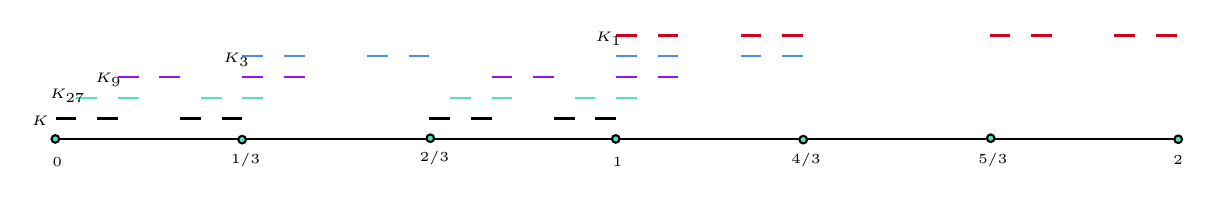
\begin{tikzpicture}[x=0.75pt,y=0.75pt,yscale=-1,xscale=1]
		%uncomment if require: \path (0,300); %set diagram left start at 0, and has height of 300
		
		%Straight Lines [id:da3663042093379123] 
		\draw    (70,160) -- (340,160) ;
		%Straight Lines [id:da30548704278309113] 
		\draw [color={rgb, 255:red, 144; green, 19; blue, 254 }  ,draw opacity=1 ][fill={rgb, 255:red, 144; green, 19; blue, 254 }  ,fill opacity=1 ]   (100,130) -- (110,130) ;
		%Straight Lines [id:da6192529867444463] 
		\draw [color={rgb, 255:red, 144; green, 19; blue, 254 }  ,draw opacity=1 ][fill={rgb, 255:red, 144; green, 19; blue, 254 }  ,fill opacity=1 ]   (120,130) -- (130,130) ;
		%Straight Lines [id:da9732533945560831] 
		\draw [color={rgb, 255:red, 144; green, 19; blue, 254 }  ,draw opacity=1 ][fill={rgb, 255:red, 144; green, 19; blue, 254 }  ,fill opacity=1 ]   (160,130) -- (170,130) ;
		%Straight Lines [id:da3271016125124977] 
		\draw [color={rgb, 255:red, 144; green, 19; blue, 254 }  ,draw opacity=1 ][fill={rgb, 255:red, 144; green, 19; blue, 254 }  ,fill opacity=1 ]   (180,130) -- (190,130) ;
		%Straight Lines [id:da21707011590164038] 
		\draw [color={rgb, 255:red, 144; green, 19; blue, 254 }  ,draw opacity=1 ][fill={rgb, 255:red, 144; green, 19; blue, 254 }  ,fill opacity=1 ]   (280,130) -- (290,130) ;
		%Straight Lines [id:da6944131266707991] 
		\draw [color={rgb, 255:red, 144; green, 19; blue, 254 }  ,draw opacity=1 ][fill={rgb, 255:red, 144; green, 19; blue, 254 }  ,fill opacity=1 ]   (300,130) -- (310,130) ;
		%Straight Lines [id:da4699188203805358] 
		\draw [color={rgb, 255:red, 144; green, 19; blue, 254 }  ,draw opacity=1 ][fill={rgb, 255:red, 144; green, 19; blue, 254 }  ,fill opacity=1 ]   (340,130) -- (350,130) ;
		%Straight Lines [id:da4206242986397042] 
		\draw [color={rgb, 255:red, 144; green, 19; blue, 254 }  ,draw opacity=1 ][fill={rgb, 255:red, 144; green, 19; blue, 254 }  ,fill opacity=1 ]   (360,130) -- (370,130) ;
		%Straight Lines [id:da18149657347980463] 
		\draw    (340,160) -- (610,160) ;
		%Shape: Circle [id:dp0666096192315917] 
		\draw  [fill={rgb, 255:red, 80; green, 227; blue, 194 }  ,fill opacity=1 ] (338,159.83) .. controls (338,158.82) and (338.82,158) .. (339.83,158) .. controls (340.85,158) and (341.67,158.82) .. (341.67,159.83) .. controls (341.67,160.85) and (340.85,161.67) .. (339.83,161.67) .. controls (338.82,161.67) and (338,160.85) .. (338,159.83) -- cycle ;
		%Shape: Circle [id:dp9884226065274095] 
		\draw  [fill={rgb, 255:red, 80; green, 227; blue, 194 }  ,fill opacity=1 ] (609,160) .. controls (609,158.99) and (609.82,158.17) .. (610.83,158.17) .. controls (611.85,158.17) and (612.67,158.99) .. (612.67,160) .. controls (612.67,161.01) and (611.85,161.83) .. (610.83,161.83) .. controls (609.82,161.83) and (609,161.01) .. (609,160) -- cycle ;
		%Shape: Circle [id:dp4266605000657435] 
		\draw  [fill={rgb, 255:red, 80; green, 227; blue, 194 }  ,fill opacity=1 ] (68,159.83) .. controls (68,158.82) and (68.82,158) .. (69.83,158) .. controls (70.85,158) and (71.67,158.82) .. (71.67,159.83) .. controls (71.67,160.85) and (70.85,161.67) .. (69.83,161.67) .. controls (68.82,161.67) and (68,160.85) .. (68,159.83) -- cycle ;
		%Straight Lines [id:da9770401267799609] 
		\draw    (70,150) -- (80,150) ;
		%Straight Lines [id:da04489044686774091] 
		\draw    (90,150) -- (100,150) ;
		%Straight Lines [id:da6941262785413165] 
		\draw    (130,150) -- (140,150) ;
		%Straight Lines [id:da5194844297129821] 
		\draw    (150,150) -- (160,150) ;
		%Straight Lines [id:da7760536614328373] 
		\draw    (250,150) -- (260,150) ;
		%Straight Lines [id:da3062585649045857] 
		\draw    (270,150) -- (280,150) ;
		%Straight Lines [id:da9561569076239738] 
		\draw    (310,150) -- (320,150) ;
		%Straight Lines [id:da058965052347594415] 
		\draw    (330,150) -- (340,150) ;
		%Straight Lines [id:da08135691890618824] 
		\draw [color={rgb, 255:red, 80; green, 227; blue, 194 }  ,draw opacity=1 ]   (80,140) -- (90,140) ;
		%Straight Lines [id:da9319257229221587] 
		\draw [color={rgb, 255:red, 80; green, 227; blue, 194 }  ,draw opacity=1 ]   (100,140) -- (110,140) ;
		%Straight Lines [id:da7931772700043691] 
		\draw [color={rgb, 255:red, 80; green, 227; blue, 194 }  ,draw opacity=1 ]   (140,140) -- (150,140) ;
		%Straight Lines [id:da9644967110186122] 
		\draw [color={rgb, 255:red, 80; green, 227; blue, 194 }  ,draw opacity=1 ]   (160,140) -- (170,140) ;
		%Straight Lines [id:da7254332920147846] 
		\draw [color={rgb, 255:red, 80; green, 227; blue, 194 }  ,draw opacity=1 ]   (260,140) -- (270,140) ;
		%Straight Lines [id:da9189177324927327] 
		\draw [color={rgb, 255:red, 80; green, 227; blue, 194 }  ,draw opacity=1 ]   (280,140) -- (290,140) ;
		%Straight Lines [id:da000462332081352157] 
		\draw [color={rgb, 255:red, 80; green, 227; blue, 194 }  ,draw opacity=1 ]   (320,140) -- (330,140) ;
		%Straight Lines [id:da36078056296552363] 
		\draw [color={rgb, 255:red, 80; green, 227; blue, 194 }  ,draw opacity=1 ]   (340,140) -- (350,140) ;
		%Straight Lines [id:da5133848731279023] 
		\draw [color={rgb, 255:red, 74; green, 144; blue, 226 }  ,draw opacity=1 ]   (160,120) -- (170,120) ;
		%Straight Lines [id:da4451939796286255] 
		\draw [color={rgb, 255:red, 74; green, 144; blue, 226 }  ,draw opacity=1 ]   (180,120) -- (190,120) ;
		%Straight Lines [id:da43204946632563] 
		\draw [color={rgb, 255:red, 74; green, 144; blue, 226 }  ,draw opacity=1 ]   (220,120) -- (230,120) ;
		%Straight Lines [id:da7906473674904837] 
		\draw [color={rgb, 255:red, 74; green, 144; blue, 226 }  ,draw opacity=1 ]   (240,120) -- (250,120) ;
		%Straight Lines [id:da04579659517201762] 
		\draw [color={rgb, 255:red, 74; green, 144; blue, 226 }  ,draw opacity=1 ]   (340,120) -- (350,120) ;
		%Straight Lines [id:da25232261478749574] 
		\draw [color={rgb, 255:red, 74; green, 144; blue, 226 }  ,draw opacity=1 ]   (360,120) -- (370,120) ;
		%Straight Lines [id:da034179599778776604] 
		\draw [color={rgb, 255:red, 74; green, 144; blue, 226 }  ,draw opacity=1 ]   (400,120) -- (410,120) ;
		%Straight Lines [id:da778496809035435] 
		\draw [color={rgb, 255:red, 74; green, 144; blue, 226 }  ,draw opacity=1 ]   (420,120) -- (430,120) ;
		%Straight Lines [id:da3950412348752457] 
		\draw [color={rgb, 255:red, 208; green, 2; blue, 27 }  ,draw opacity=1 ]   (340,110) -- (350,110) ;
		%Straight Lines [id:da9542539719446077] 
		\draw [color={rgb, 255:red, 208; green, 2; blue, 27 }  ,draw opacity=1 ]   (360,110) -- (370,110) ;
		%Straight Lines [id:da975939203402955] 
		\draw [color={rgb, 255:red, 208; green, 2; blue, 27 }  ,draw opacity=1 ]   (400,110) -- (410,110) ;
		%Straight Lines [id:da6837814611254798] 
		\draw [color={rgb, 255:red, 208; green, 2; blue, 27 }  ,draw opacity=1 ]   (420,110) -- (430,110) ;
		%Straight Lines [id:da1335307904306704] 
		\draw [color={rgb, 255:red, 208; green, 2; blue, 27 }  ,draw opacity=1 ]   (520,110) -- (530,110) ;
		%Straight Lines [id:da6855728787535145] 
		\draw [color={rgb, 255:red, 208; green, 2; blue, 27 }  ,draw opacity=1 ]   (540,110) -- (550,110) ;
		%Straight Lines [id:da26557145189620557] 
		\draw [color={rgb, 255:red, 208; green, 2; blue, 27 }  ,draw opacity=1 ]   (580,110) -- (590,110) ;
		%Straight Lines [id:da4074209351984093] 
		\draw [color={rgb, 255:red, 208; green, 2; blue, 27 }  ,draw opacity=1 ]   (600,110) -- (610,110) ;
		%Shape: Circle [id:dp983839454545631] 
		\draw  [fill={rgb, 255:red, 80; green, 227; blue, 194 }  ,fill opacity=1 ] (158,160.17) .. controls (158,159.15) and (158.82,158.33) .. (159.83,158.33) .. controls (160.85,158.33) and (161.67,159.15) .. (161.67,160.17) .. controls (161.67,161.18) and (160.85,162) .. (159.83,162) .. controls (158.82,162) and (158,161.18) .. (158,160.17) -- cycle ;
		%Shape: Circle [id:dp44575128451386936] 
		\draw  [fill={rgb, 255:red, 80; green, 227; blue, 194 }  ,fill opacity=1 ] (248.67,159.5) .. controls (248.67,158.49) and (249.49,157.67) .. (250.5,157.67) .. controls (251.51,157.67) and (252.33,158.49) .. (252.33,159.5) .. controls (252.33,160.51) and (251.51,161.33) .. (250.5,161.33) .. controls (249.49,161.33) and (248.67,160.51) .. (248.67,159.5) -- cycle ;
		%Shape: Circle [id:dp038392589885732686] 
		\draw  [fill={rgb, 255:red, 80; green, 227; blue, 194 }  ,fill opacity=1 ] (428.33,160.17) .. controls (428.33,159.15) and (429.15,158.33) .. (430.17,158.33) .. controls (431.18,158.33) and (432,159.15) .. (432,160.17) .. controls (432,161.18) and (431.18,162) .. (430.17,162) .. controls (429.15,162) and (428.33,161.18) .. (428.33,160.17) -- cycle ;
		%Shape: Circle [id:dp0834667196596044] 
		\draw  [fill={rgb, 255:red, 80; green, 227; blue, 194 }  ,fill opacity=1 ] (518.67,159.5) .. controls (518.67,158.49) and (519.49,157.67) .. (520.5,157.67) .. controls (521.51,157.67) and (522.33,158.49) .. (522.33,159.5) .. controls (522.33,160.51) and (521.51,161.33) .. (520.5,161.33) .. controls (519.49,161.33) and (518.67,160.51) .. (518.67,159.5) -- cycle ;
		
		% Text Node
		\draw (67,167.4) node [anchor=north west][inner sep=0.75pt]  [font=\tiny]  {$0$};
		% Text Node
		\draw (337,167.4) node [anchor=north west][inner sep=0.75pt]  [font=\tiny]  {$1$};
		% Text Node
		\draw (607,166.4) node [anchor=north west][inner sep=0.75pt]  [font=\tiny]  {$2$};
		% Text Node
		\draw (153,165.4) node [anchor=north west][inner sep=0.75pt]  [font=\tiny]  {$1/3$};
		% Text Node
		\draw (244,164.4) node [anchor=north west][inner sep=0.75pt]  [font=\tiny]  {$2/3$};
		% Text Node
		\draw (423,165.4) node [anchor=north west][inner sep=0.75pt]  [font=\tiny]  {$4/3$};
		% Text Node
		\draw (513,165.4) node [anchor=north west][inner sep=0.75pt]  [font=\tiny]  {$5/3$};
		% Text Node
		\draw (57,147.4) node [anchor=north west][inner sep=0.75pt]  [font=\tiny]  {$K$};
		% Text Node
		\draw (65.67,134.07) node [anchor=north west][inner sep=0.75pt]  [font=\tiny]  {$K_{27}$};
		% Text Node
		\draw (87.67,126.4) node [anchor=north west][inner sep=0.75pt]  [font=\tiny]  {$K_{9}$};
		% Text Node
		\draw (149.33,117.07) node [anchor=north west][inner sep=0.75pt]  [font=\tiny]  {$K_{3}$};
		% Text Node
		\draw (328.67,106.73) node [anchor=north west][inner sep=0.75pt]  [font=\tiny]  {$K_{1}$};
		
		
	\end{tikzpicture}
\end{figure}
	\FloatBarrier
\end{solution}
\begin{remark}
	Note that $ K \oplus K = \bigcup_{x\in K}( K \oplus x) = [0,2] $. I.e. the set of all numbers that can be created by adding two Cantor numbers is all the numbers in $ [0,2] $. Note that the Cantor set has Lebesgue measure zero, however $ [0,2] $ has measure 2. That is because $ \bigcup_{x\in K}) $ is in fact an uncountable union of sets (since a Cantor set is uncountable).
\end{remark}

\begin{problem}
	Let $ \Omega $ be a finite non-empty set, and let $ \mathcal{I} $ consist of all singletons in $ \Omega $, together with $ \emptyset $ and $ \Omega $. Let $ p: \Omega \to [0,1] $ with $ \sum_{\omega \in \Omega}p(\omega) = 1 $, and define $ \prob(\emptyset) = 0,\prob(\Omega) = 1 $, and $ \prob\set{\omega}=\prob(w) $ for all $ \omega \in \Omega $.
	\begin{enumerate}[(a)]
		\item Prove that $ \mathcal{I} $ is a semialgebra.
		\item Prove that (2.3.2) and $ (2.3.3) $ are satisfied. 
		\item Describe precisely the $ \mathcal{M} $ and $ \prob^* $ that result from applying Theorem 2.3.1 in Rosenthal.
		\item Are these $ \mathcal{M} $ and $ \prob^* $ the same as those described in Theorem 2.2.1 in Rosenthal?
 	\end{enumerate}
\end{problem}
\begin{solution}
	\begin{enumerate}[(a)]
		\item By definition $ \mathcal{I} $ contains $ \emptyset $ and well as $ \Omega $. $ \mathcal{I} $ is also closed under finite intersection as the intersection of two singletons is either a singleton or the empty set, and the intersection of $ \Omega $ with any singleton is a singleton. Furthermore, the intersection of any singleton with empty set is the empty set that is contained in $ \mathcal{I} $. Finally, let $ E \in \mathcal{I} $. If $ E $ is either $ \Omega $ or the empty set, then it complement can trivially be written as the disjoint union of $ \emptyset $ or $ \Omega $ respectively. If $ E $ is a singleton, then $ E^c $ can be written as the disjoint union of the singleton of its elements. Thus $ \mathcal{I} $ is a semialgebra.
		
		\item To check $ (2.3.2) $ let $ A_1,\cdots,A_k \in \mathcal{I} $ disjoint with $ \bigcup_i A_i \in \mathcal{I} $. Then $ \bigcup_i A_i = \Omega $ the collection $ A_i $'s are all of the singletons. Thus 
		\[ 1 = \prob(\bigcup_i A_i) = \prob(\Omega) = \sum_i \prob(A_i) = \sum_{\omega\in\Omega}\prob(\set{\omega}) = \sum_{\omega\in\Omega}p(\omega) = 1. \]
		Thus $ 2.3.2 $ holds with equality
		
		\noindent To verify $ (2.3.3) $ let $ A,A_1,A_2,\cdots,A_k \in \mathcal{I} $ with $ A \subset \bigcup_i A_i $. If $ A $ is empty set, then (2.3.3) holds as $ 0 \leq a $ for all $ a\in [0,1] $. If $ A $ is $ \Omega $, then the the sets $ A_i $ are the sets of all singletons. Thus 2.3.3 holds as $ 1\leq 1 $. Lastly, if $ A $ is a singleton, then at least one of $ A_i $'s should be the same as $ A $. Then $ \prob(A) \leq \prob(A_1) + \cdots + \prob(A_j) +  \cdots + \prob(A_k) $ for some $ 0\leq j \leq n $. Since $ \prob(A_j) = \prob(A) $ then 2.3.3 holds.
		
		\item The collection $ \mathcal{M} $ will be the same as the power set of $ \Omega $. And the probability measure $ \prob^* $ will be give as
		\[ \prob^*(A) = \sum_{\omega\in A} p(\omega). \]
		
		\item Although $ \mathcal{M} $ is the same as in theorem $ 2.3.1 $, but $ \prob^* $ is not the same. The probability measure defined in Theorem 2.3.1 is the uniform probability measure, where here it is not. The probability measure $ \prob^* $ is a more general one and will be the same as probability measure in Theorem 2.3.1 if we choose $ p(\omega) = 1/\abs{\Omega} $.
	\end{enumerate}
\end{solution}

\begin{problem}
	Let $ \prob $ and $ \mathbb{Q} $ be two probability measures defined on the same sample space $ \Omega $ and $\sigma\text{-algebra}$ $ \mathcal{F} $. 
	\begin{enumerate}[(a)]
		\item Suppose that $ \prob(A) = \mathbb{Q}(A) $ for all $ A \in \mathcal{F} $ with $ \prob(A) \leq 1/2 $. Prove that $ \prob = \mathbb{Q} $, i.e. that $ \prob(A) = \mathbb{Q}(A) $ for all $ A \in \mathcal{F} $.
		\item Give an example where $ \prob(A) = \qrob(A) $ for all $ A \in \mathcal{F} $ with $ \prob(A)<1/2 $, such that $ \prob \neq \qrob $, i.e. that $ \prob(A) \neq \qrob(A) $ for some $ A \in \mathcal{F} $.
	\end{enumerate}
\end{problem}
\begin{solution}
	\begin{enumerate}[(a)]
		\item Let $ A \in \mathcal{F} $ with $ \prob(A) > 1/2 $, hence $ \prob(A^c) \leq 1/2 $. Also, let $ E \in\mathcal{F} $ such that $ \prob(E)\leq 1/2 $. By definition (by using 2.3.7 or using the fact that $ \mathcal{F} $ is a $\sigma\text{-algebra}$ thus closed under intersection and complement) we can write
		\[ \prob(A) = \prob(A \cap E) + \prob(A\cap E^c). \]
		Observe that $ A\cap E \subseteq E $ thus by monotonicity $ \prob(A\cap E) \leq \prob(E) \leq 1/2 $. Further more, we can write $ \prob(A\cap E^c) = 1 - \prob(A^c \cup E) $. For the second term in the RHS we have
		\[ \prob(A^c \cup E) = \prob(A^c) + \prob(E) - \prob(A^c\cap E). \]
		Note that $ \prob(A^c)\leq 1/2 $ as well as since $ A^c\cap E \subset A^c $ thus by monotonicity $ \prob(A^c\cap E) \leq \prob(A^c) \leq 1/2 $. Thus
		\[ \prob(A) = \prob(A\cap E) + 1 - \prob(A^c) - \prob(E) + \prob(A^c\cap E). \]
		For all the terms in the RHS, since their measure with respect to $ \prob $ is less than oe equal to $ 1/2 $, thus $ \prob $ and $ \qrob $ agrees on them. Thus 
		\[ \prob(A) = \qrob(A\cap E) + 1 - \qrob(A^c) - \qrob(E) + \qrob(A^c\cap E) = \qrob(A). \]
		This completes the proof.
		
		\noindent \textbf{An easier solution}. Let $ A \in \mathcal{F} $ with $ \prob(A) > 1/2 $. Then $ \prob(A) = 1 - \prob(A^c) = 1 - \qrob(A^c) = \qrob(A) $, where we used the fact that $ \prob(A^c)\leq 1/2 $ thus $ \prob(A^c) = \qrob(A^c) $.
		
		\item Let $ \Omega =  \set{1,2} $ with $ \mathcal{F} $ being the power set of $ \Omega $. Then defined
		\[ \prob(\emptyset) = 0, \quad \prob(\set{1}) = \prob(\set{2}) = 1/2, \quad \prob(\set{1,2}) = 1. \]
		And
		\[ \qrob(\emptyset) = 0, \quad \qrob(\set{1}) = 1/10, \quad \qrob(\set{2})=9/10, \quad \qrob(\set{1,2}) = 1. \]
	\end{enumerate}
\end{solution}
\begin{remark}
	The hypothesis in part (a) in question above means that $ \prob $ and $ \qrob $ on all of the sets that has measure less than or equal to 1/2 w.r.t $ \prob $, must agree on all of the element of $ \mathcal{F} $.
\end{remark}

\begin{problem}
	Let $ (\Omega_1,\mathcal{F}_1,\prob_1) $ be Lebesgue measure on $ [0,1] $. Consider a second probability triple $ (\Omega_2, \mathcal{F}_2, \prob_2) $, defined as follows: $ \Omega_2 = \set{1,2} $, $ \mathcal{F}_2 $ consists of all subsets of $ \Omega_2 $, and $ \prob_2 $ is defined by $ \prob_2\set{1} = 1/3 $ and $ \prob_2\set{2} = 2/3 $, and additivity. Let $ (\Omega,\mathcal{F},\prob) $ be the product measure of $ (\Omega_1, \mathcal{F}_1, \prob_1) $ and $ (\Omega_2,\mathcal{F_2},\prob_2) $.
	\begin{enumerate}[(a)]
		\item Express each of $ \Omega, \mathcal{F} $ and $ \prob $ as explicitly as possible.
		\item Find a set $ A \in \mathcal{F} $ such that $ \prob(A) = 3/4 $.
	\end{enumerate}
\end{problem}
\begin{solution}
	\begin{enumerate}[(a)]
		\item The set $ \Omega $ is 
		\[ \Omega = \set{1,2}\times [0,1]. \]
		The collection $ \mathcal{F} $ is given by
		\[ \mathcal{F} = \set{\set{1}\times B: B \in\mathcal{B}}\quad \cup\quad \set{\set{2}\times B: B \in \mathcal{B}} \quad\cup\quad \set{\set{1,2}\times B: B \in \mathcal{B}}. \]
		And $ \prob $ is given by
		\[ \prob(\set{1}\times B) = \lambda(B)/3,\quad \prob(\set{2}\times B) = 2\lambda(B)/3,\quad \prob(\set{1,2}\times B) = \lambda(B). \]
		\item One easy choice for such a set would be $ A = \set{1,2}\times(0,3/4) $.
	\end{enumerate}
\end{solution}
\newpage


\section{Further Probabilistic Foundations}
\begin{problem}
	Let $ X $ be a real-valued random variable defined on a probability triple $ (\Omega, \mathcal{F},\prob) $. Fill in the following blanks:
	\begin{enumerate}[(a)]
		\item $ \mathcal{F} $ is a collection of subsets of \blank.
		\item $ \prob(A) $ is a well-defined element of \blank provided that $ A $ is an element of \blank.
		\item $ \set{X\leq 5} $ is shorthand notation for the particular subset of \blank which is defined \blank.
		\item If $ S $ is a subset of \blank, then $ \set{X\in S} $ is a subset of \blank.
		\item If $ S $ is a \blank subset of \blank, then $ \set{X \in S} $ must be a element of \blank.
	\end{enumerate}
\end{problem}

